\chapter{Основная часть}

\section{Краткое описание этапов работы}

Разрабатываемая система предназначена для интеграции в путеизмерительную тележку и должна обеспечивать высокоточные измерения в реальном времени при минимальном вмешательстве оператора. Разработка такой системы представляет собой комплексную инженерную задачу, требующую согласованного создания аппаратных и программных компонентов.

Управляющим ядром системы выступил микроконтроллер STM32 F303VCT6 в составе отладочной платы STM32F3 DISCOVERY. Выбор был обусловлен оптимальным сочетанием вычислительной мощности и необходимой периферии. Ядро ARM Cortex-M4 с поддержкой аппаратных операций с плавающей точкой и тактовой частотой до 72 МГц обеспечивает достаточную производительность для реализации алгоритмов фильтрации и обработки данных с датчиков в реальном времени. Критически важным фактором стало наличие на самой плате интегрированных МЕМС-датчиков: трёхосевого гироскопа L3GD20 и комбинированного модуля LSM303DLHC, включающий в себя акселерометр, магнитометр и температурный датчик. Кроме того, микроконтроллер обладает широким набором встроенных интерфейсов: ADC, DAC, таймеры, USART, SPI, I2C, что упрощает подключение дополнительной внешней периферии и коммуникацию с верхним уровнем системы.

Основные этапы разработки системы включают:

\begin{enumerate}
	\item Разработка низкоуровневого ПО для микроконтроллера;	
	\item Разработка алгоритмов фильтрации данных;	
	\item Создание графического интерфейса пользователя;	
	\item Разработка ПО для постобработки данных;
	\item Проектирование печатной платы;
	\item Конструирование корпуса прибора;	
	\item Комплексные испытания.
\end{enumerate}

% -----------------------------------------------------------------------------

\section{Разработка низкоуровневого ПО для МК}
\label{sec:firmware}

Разработка низкоуровневого программного обеспечения (прошивки) была направлена на создание базового функционала системы: сбор данных с датчиков, их первичную обработку и организацию надёжного двустороннего обмена данными с персональным компьютером через интерфейс USB. Конкретными задачами являлись инициализация аппаратных модулей МК, реализация драйверов для гироскопа L3GD20 и комбинированного датчика LSM303DLHC, организация циклического опроса сенсоров, а также создание протокола для передачи телеметрии и приёма управляющих команд.

Разработка велась на языках С и С++, что соответствует отраслевым стандартам для встраиваемых систем благодаря высокой эффективности и низкоуровневому контролю. В качестве основы для работы с периферией микроконтроллера использовалась библиотека стандартной периферии (Standard Periphery Library, SPL) от STMicroelectronics. Данная библиотека предоставляет структурированный набор функций для конфигурации всех встроенных модулей МК, что ускоряет разработку, сохраняя прозрачность управления аппаратными ресурсами.
\section{Разработка алгоритмов фильтрации данных}

исследование и реализация методов обработки сигналов с акселерометра и гироскопа, направленных на компенсацию шумов, дрейфа нуля и совмещение данных для точного определения пространственного положения.
\section{Создание графического интерфейса пользователя}
\label{sec:gui}

Для обеспечения удобного взаимодействия оператора с измерительной системой и контроля процесса измерений в реальном времени было разработано специализированное клиентское приложение с графическим интерфейсом пользователя.

К разрабатываемому интерфейсу были сформулированы функциональные требования, указанные ниже.

Управление подключением и настройками: Возможность выбора последовательного порта, к которому подключён микроконтроллер, а также выбора директории и шаблона имени для сохранения файлов с данными.

Двусторонняя коммуникация с МК: Отправка управляющих команд (начало/остановка измерений, перезагрузка) и приём телеметрии в реальном времени.

Визуализация данных: Отображение текущих показаний со всех датчиков (акселерометр, гироскоп) в удобной форме, например, в виде таблицы или простых индикаторов, для оперативной оценки работоспособности системы.

Управление процессом измерений: Предоставление интуитивно понятных элементов управления (кнопки) для запуска и завершения сеанса измерений, а также для выполнения вспомогательных операций, таких как привязка к координатам GPS.

Формирование лога событий: Наличие информационной панели для отображения статусных сообщений, ошибок и подтверждения выполненных действий.


\begin{figure}[ht]
	\centering
	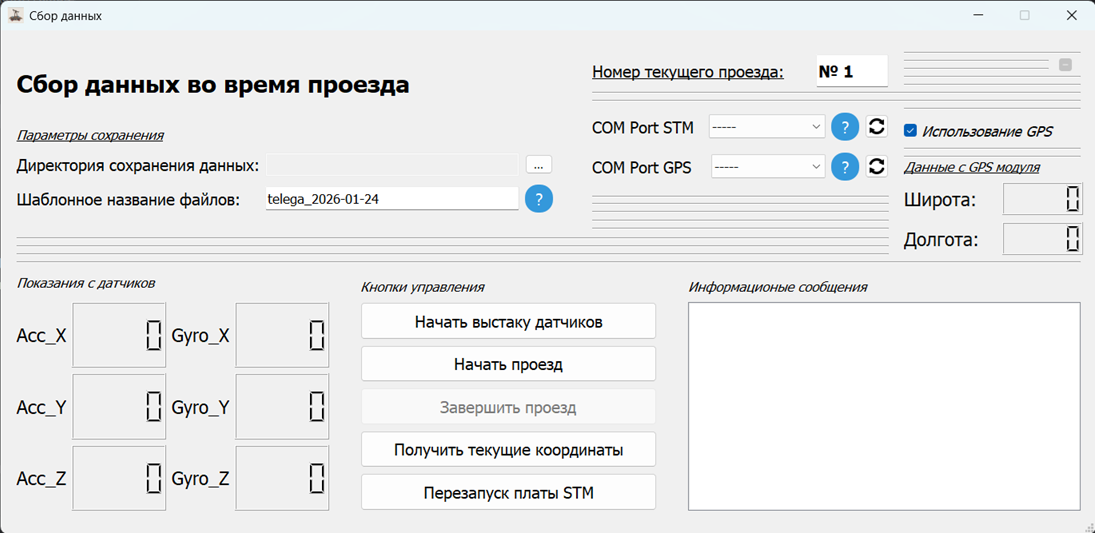
\includegraphics[width=0.9\textwidth]{images/main_part/GUI.png}
	\caption{Разработанный графический интерфейс программы}
	\label{picture:GUI}
\end{figure}

Разработанное приложение, внешний вид которого представлен на рис. \ref{picture:GUI}, полностью удовлетворяет перечисленным требованиям. Его интерфейс логически разделён на несколько функциональных зон:

\begin{itemize}
	\item Секция параметров сохранения (поля для указания пути сохранения данных и шаблона имени файлов, что обеспечивает структурированное хранение результатов каждого проезда);
	\item Секция управления подключением (элементы для выбора COM-портов микроконтроллера и GPS-модуля, а также переключатель активации использования геопозиционных данных);	
	\item Панель визуализации данных в реальном времени (таблица для отображения текущих значений с акселерометра и гироскопа).
	\item Панель управления (группа кнопок для всех ключевых действий: «Начать выставку датчиков» (калибровка), «Начать проезд», «Завершить проезд», «Получить текущие координаты» и «Перезапуск платы STM»);
	\item Область информационных сообщений (Текстовое поле, выполняющее роль лога событий, для вывода служебной информации и диагностики).
\end{itemize}

Приложение реализовано на языке Python с использованием фреймворка PyQt5 для создания производительного и кроссплатформенного графического интерфейса. Выбор PyQt5 обусловлен его мощными возможностями для создания сложных интуитивных интерфейсов, стабильной работой и простой интеграцией с библиотеками для последовательной связи (PySerial) и научных вычислений (NumPy), что в совокупности обеспечило требуемую функциональность и надёжность.





\section{Разработка ПО для постобработки данных}

Для получения геометрических параметров железнодорожного пути необходимо выполнить обработку записанных массивов инерциальных данных с применением навигационного алгоритма, описанного в разделе \ref{sec:nav_algoritm}. С этой целью в рамках проекта было разработано специализированное программное обеспечение для постобработки данных.

Программный комплекс реализует следующие функции:

\begin{itemize}
	\item загрузка и анализ бинарных логов, сформированных микроконтроллером во время измерительного проезда;
	\item выполнение полного навигационного расчёта траектории в соответствии с математическим аппаратом, изложенным в разд. 5.7;
	\item визуализацию результатов в виде графиков временных рядов полученных и рассчитанных массивов величин;
	\item формирование структурированных отчётов для последующего анализа и паспортизации участков пути.
\end{itemize}

Архитектура приложения построена по модульному принципу, что позволяет легко добавлять новые методы обработки и адаптировать алгоритмы под требуемые задачи. Реализация выполнена на языке Python с применением готовых библиотек (NumPy, Matplotlib), что обеспечивает гибкость разработки и удобство сопровождения кода.
\section{Проектирование печатной платы}

разработка схемы и трассировка платы для обеспечения стабильного питания микроконтроллера и подключения периферийных модулей таких как GPS-приёмник, датчик пройденного пути и прочее.
\section{Конструирование корпуса прибора}
\label{sec:enclosure}

проектирование защитного корпуса прибора, учитывающего условия эксплуатации на железной дороге, требования эргономики и охлаждения электронных компонентов.
\section{Комплексные испытания}

проведение тестов разработанной системы для верификации точности измерений, оценки надёжности и соответствия техническому заданию.









